\documentclass[11pt]{article}

% \VignetteIndexEntry{Getting Started with Spatstat}

\usepackage{graphicx}
\usepackage{anysize}
\marginsize{2cm}{2cm}{2cm}{2cm}

\newcommand{\pkg}[1]{\texttt{#1}}
\newcommand{\bold}[1]{{\textbf {#1}}}
\newcommand{\R}{{\sf R}}
\newcommand{\spst}{\pkg{spatstat}}
\newcommand{\Spst}{\pkg{Spatstat}}

\usepackage{Sweave}
\begin{document}
\Sconcordance{concordance:Intro.tex:Intro.Rnw:1 3 1 1 4 11 1 1 0 6 1 1 15 14 1 1 4 1 %
8 1 2 6 1 1 2 1 0 2 1 1 5 4 0 1 5 7 0 1 2 5 1 1 13 15 0 1 2 3 1 1 2 28 %
0 2 2 11 0 2 2 7 0 2 2 8 0 1 2 2 1 1 15 17 0 1 2 18 1}

\bibliographystyle{plain}
\thispagestyle{empty}

\setkeys{Gin}{width=0.6\textwidth}


\title{Getting started with Spatial Random Forests}
\author{Christophe A.N. Biscio}
\date{For \pkg{Rsandbox} version \texttt{0.0.0.9000}}
\maketitle



\section{Integration with \Spst}

The packate \pkg{Rsandbox} relies on \spst to work.  
For the user, it means that a point pattern must be input as a \texttt{ppp} object 
and the covariates as \texttt{im} object rather than raster.

Specifically, \pkg{Rsandbox}  depends on  \pkg{spatstat.model},
\pkg{spatstat.geom}.
In this document, we will additionally use the package \pkg{spatstat.data}
and \pkg{spatstat.random}.

\begin{Schunk}
\begin{Sinput}
> library(Rsandbox)
> library(spatstat.data)
> library(spatstat.random)
\end{Sinput}
\end{Schunk}

\section{Getting started}

We need a point pattern as a \texttt{ppp} object, 
together with a list of covariates as list of \texttt{im} objects

As an example we take the data \texttt{bei} and \texttt{bei.extra} from 
\spst. 
\begin{Schunk}
\begin{Sinput}
> par(mfrow = c(1, 3), mar = c(0, 1, 0, 0))
> plot(bei, pch=16, cex = 0.5, main = "")
> plot(bei.extra[[1]], ribbon = F, main = "")
> plot(bei.extra[[2]], ribbon = F, main = "")
\end{Sinput}
\end{Schunk}
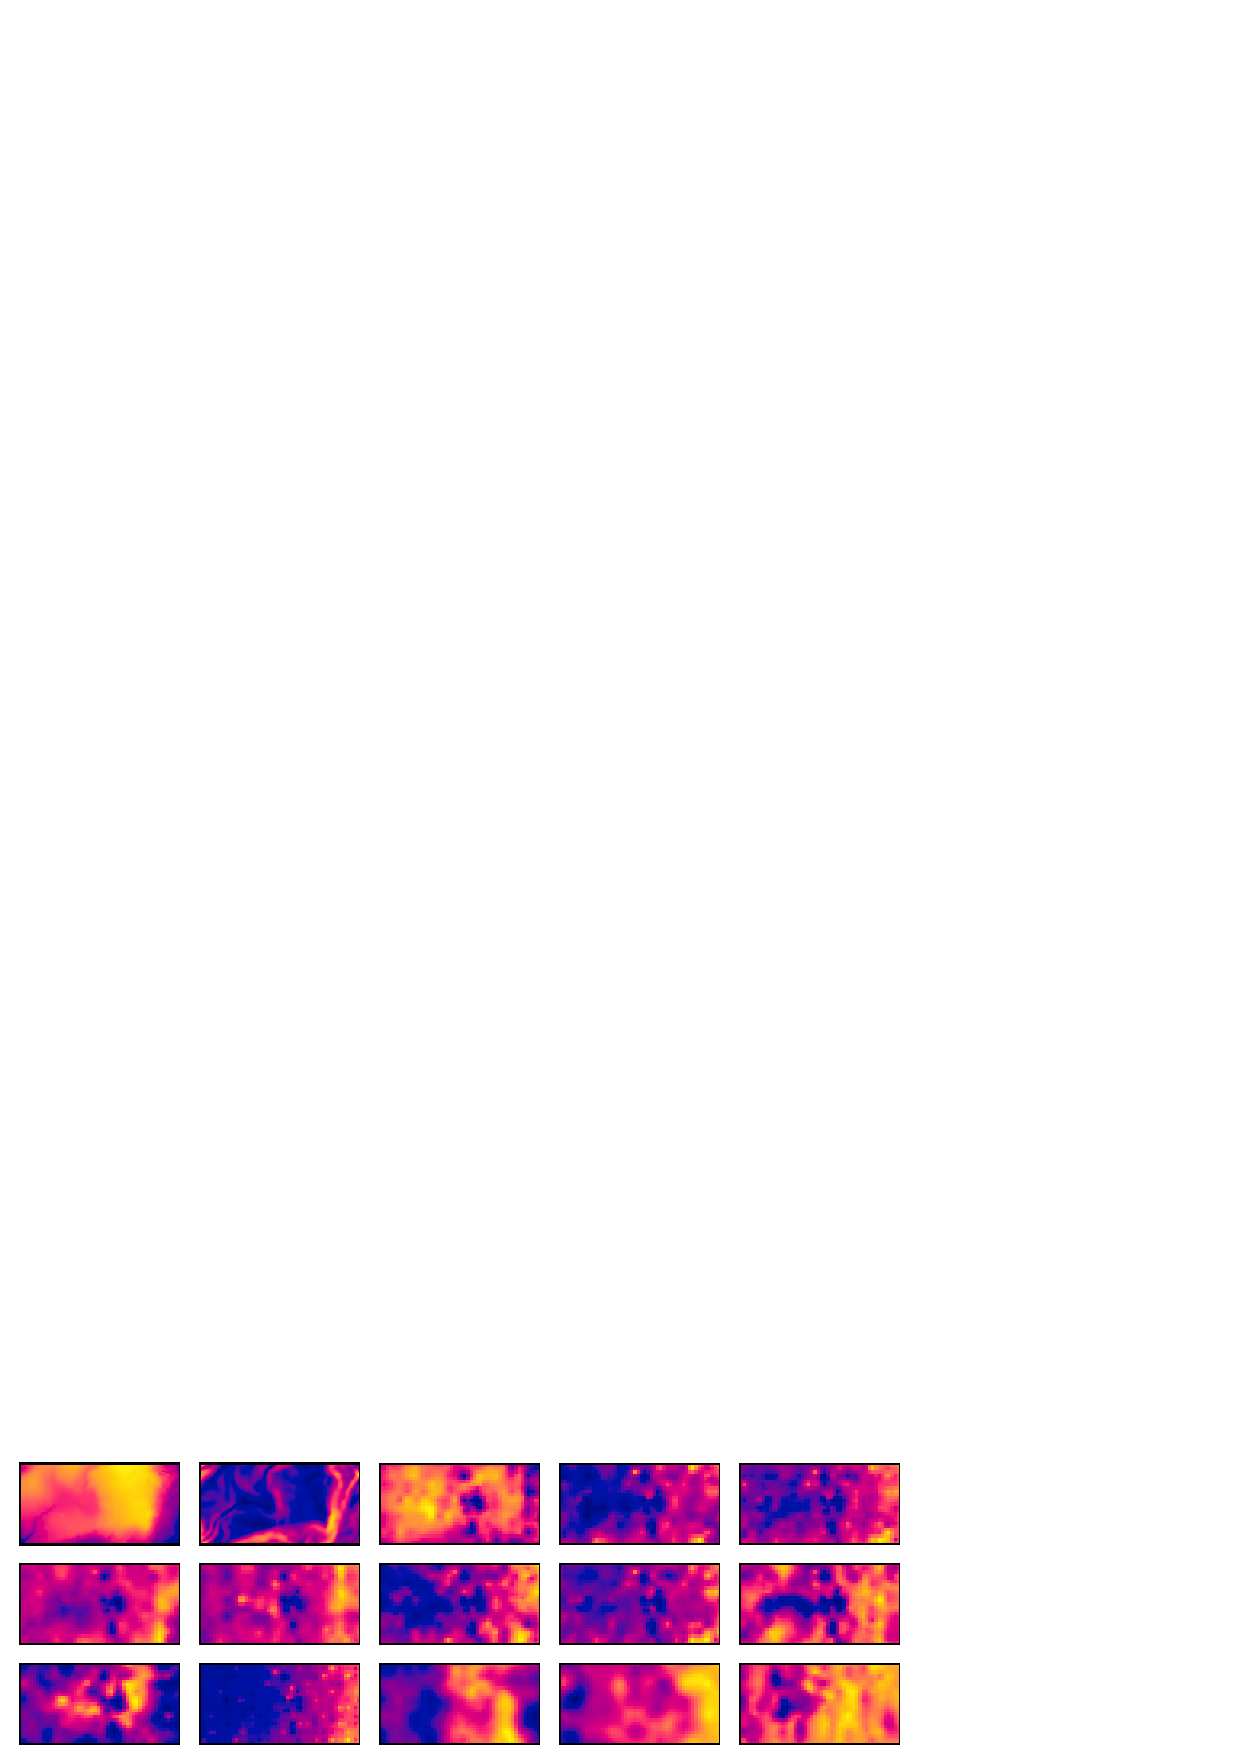
\includegraphics{Intro-003}

The function \texttt{RforestPP} generate 
a random forest intensity estimate. 

\begin{Schunk}
\begin{Sinput}
> forest <- RforestPP(
+   X = bei,
+   listcovariates = bei.extra,
+   score = "lcv2",
+   p = 0,
+   Ntree = 3,
+   mtry = 1 / 3,
+   minpts = 500,
+   cores_trees = 1
+ )
\end{Sinput}
\end{Schunk}

The arguments: 
\begin{itemize}
  \item \texttt{score} selects the score used to compare different splits. 
  From our simulations it had however a negligible impact on the results.
  \item \texttt{p} controls the thinning applied on the original point pattern 
  \texttt{X} before training an intensity tree. If $p>0$, a $p$-thinning is applied, 
  and if $p=0$, the points are bootstrapped.
  \item \texttt{Ntree} sets the number of intensity trees in the forest.
  \item \texttt{mtry}: At each split, we use a random subset of the covariates 
  where each of them is independently chosen with probability \texttt{mtry}.
  \item \texttt{minpts} is used as stopping criterion. Once the number of points 
  in a split is below \texttt{minpts}, we only allow at most one last split. 
  This ensure that we allows region where there is no points and 
  that the algorithm is not running indefinitely.
  \item \texttt{cores{\textunderscore}trees} is used of parallelisation in the sense that 
  each intensity trees computation will be allocated to a core. 
\end{itemize}

Standard \R methods have been implemented: 
\begin{itemize}
  \item to plot the estimated random forest intensity
\begin{Schunk}
\begin{Sinput}
> plot(forest)
\end{Sinput}
\end{Schunk}
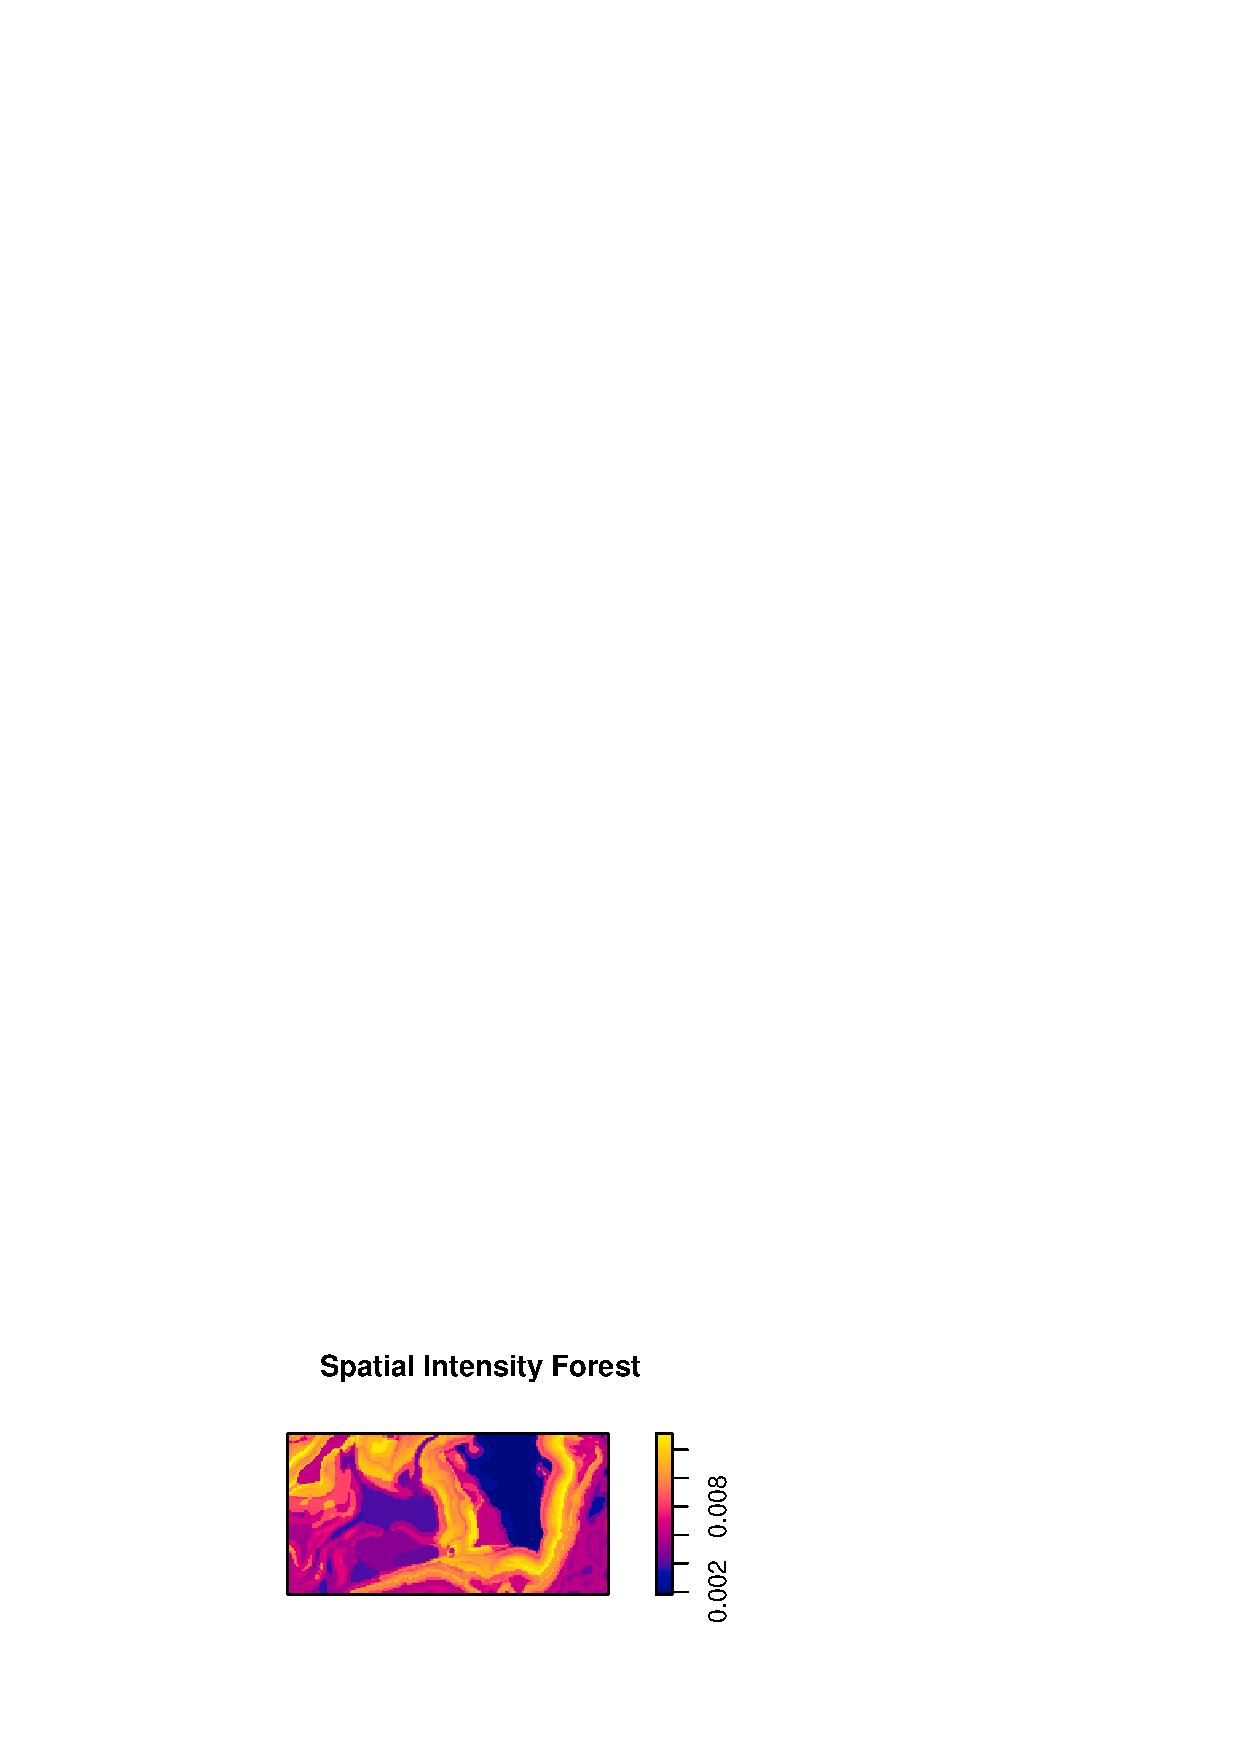
\includegraphics{Intro-005}
  \item To return the predicted intensity in new locations. There the function 
  accept the new location to be a \texttt{ppp} object 
\begin{Schunk}
\begin{Sinput}
> predict(object = forest, newdata = runifpoint(n=5, win = bei$window))
\end{Sinput}
\begin{Soutput}
[1] 0.005543827 0.007071986 0.005724216 0.009794941 0.010364657
\end{Soutput}
\end{Schunk}
or a matrix with the $x$-coordinate on the first column and the $y$-coordinate 
on the second column
\begin{Schunk}
\begin{Sinput}
> predict(object = forest, 
+         newdata = cbind(
+           runif(5, min = 0, max=1000),
+           runif(5, min = 0, max=500)))
\end{Sinput}
\begin{Soutput}
[1] 0.010715476 0.010536858 0.003894108 0.008535516 0.004037444
\end{Soutput}
\end{Schunk}
\end{itemize}


\section{Usual workflow}


When working with random intensity forest the workflow is a follow: 
\begin{itemize}
  \item In function of the available computational power, 
  choose a reasonable combination of hyperparameters: 
  \texttt{minpts},  \texttt{mtry}.
  \item Compute the Out-Of-Bag (OOB) score for a random intensity forest with 
  each combination of the hyperparameters. Select the combination with the highest OOB score.
  \item Eventually, re-run the random intensity forest with this combination of hyperparameters and 
  \texttt{Ntree} as large as possible. 
  \item Compute the variable importance (VIP) for each covariates and display the results in a plot.
\end{itemize}

\textbf{Remark:} There is in fact two more hyperparameters, \texttt{Ntree} and \texttt{p}, 
that one can choose. However, we have observed that \texttt{p} usually has a low impact on 
the mean square error. Hence we recommend to set $p=0$, meaning to boostrap the point patterns. 
Finally, \texttt{Ntree} should be chosen as large as possible, depending on the 
available computational power.

To illustrate the workflow on an example, we re-use the \texttt{bei} and \texttt{bei.extra} data.

For illustration, we will compute random intensity 
forest for all combinations of $\texttt{minpts} = 75, 100, 125$ 
and $\texttt{mtry}= 0.25, 0.5, 0.75$ with $\texttt{Ntree}=6$. 
For a more serious analyses, we should let $\texttt{minpts} = 1,2,\ldots,200$ 
and $\texttt{mtry}= 0.1,0.2,\ldots,1$, together with $\texttt{Ntree}=300$. 

\begin{Schunk}
\begin{Sinput}
> argmtry <- c(0.25, 0.5, 0.75)
> argminpts <- c(seq(75, 125, by = 25))
> allargs <- expand.grid(mtry = argmtry, minpts = argminpts)
> allargs
\end{Sinput}
\begin{Soutput}
  mtry minpts
1 0.25     75
2 0.50     75
3 0.75     75
4 0.25    100
5 0.50    100
6 0.75    100
7 0.25    125
8 0.50    125
9 0.75    125
\end{Soutput}
\end{Schunk}

We will use the \texttt{mapply} function. 

\begin{Schunk}
\begin{Sinput}
> extrarg <- list(
+   p = 0,
+   Ntree = 6,
+   cores_tree = 2,
+   X = bei,
+   listcovariates = bei.extra
+ )
> allforest <- mapply(RforestPP,
+   mtry = allargs$mtry,
+   minpts = allargs$minpts,
+   MoreArgs = extrarg,
+   SIMPLIFY = F
+ )
\end{Sinput}
\end{Schunk}

We can now compute the OOB score of all the random intensity forest above 
and choose the one with the highest score. 
\begin{Schunk}
\begin{Sinput}
> allscore <- lapply(allforest, FUN=function(i) {OOBscr(i, cores = 2)})
> allargs[which.max(allscore),]
\end{Sinput}
\begin{Soutput}
  mtry minpts
2  0.5     75
\end{Soutput}
\end{Schunk}

Then, we may, if we have the computational power, run again the code for this 
combination of parameter but with \texttt{Ntree} larger. 

\begin{Schunk}
\begin{Sinput}
> chosenforest <- RforestPP( 
+   p = 0,
+   mtry = 0.5,
+   minpts = 50,
+   Ntree = 100,
+   cores_tree = 2,
+   X = bei,
+   listcovariates = bei.extra)
\end{Sinput}
\end{Schunk}

Finally we 
\begin{itemize}
\item Visualise the estimated intensity
\begin{Schunk}
\begin{Sinput}
> plot(chosenforest)
\end{Sinput}
\end{Schunk}
\item Assessing the variable importance of each variables
\begin{Schunk}
\begin{Sinput}
> vipplot(chosenforest, sorted = T, cores = 2)
\end{Sinput}
\end{Schunk}
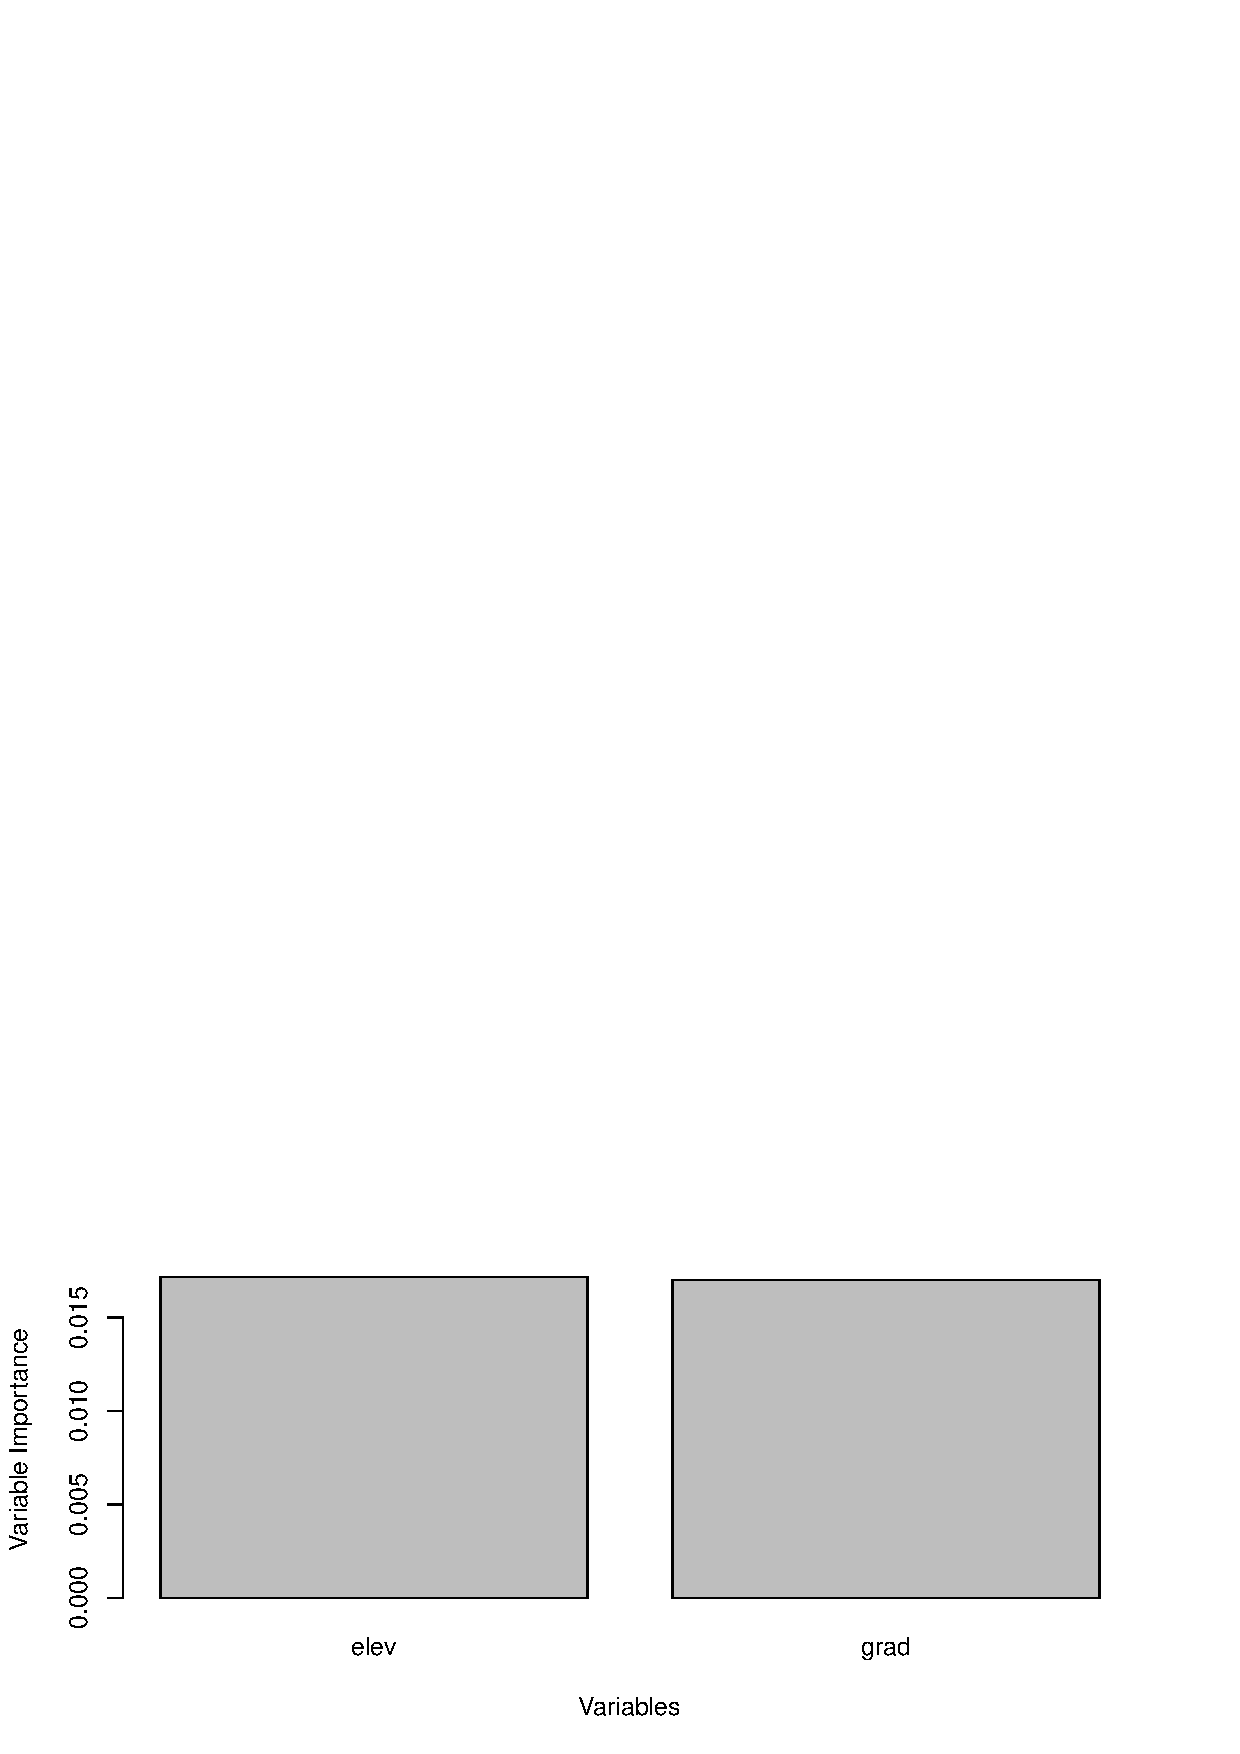
\includegraphics{Intro-013}
\end{itemize}
 


\end{document}
